% Compilar desde docs/: pdflatex -interaction=nonstopmode articulo_ieee.tex
% PENDIENTE DE PUBLICACIÓN: completar autoría/afiliación y validar extensión.
\documentclass[conference]{IEEEtran}
\usepackage[T1]{fontenc}
\usepackage[utf8]{inputenc}
\usepackage[spanish,es-tabla]{babel}
\usepackage{graphicx}
\usepackage{url}
\usepackage{amsmath}
\usepackage{booktabs}

\title{NewsScope: clasificación automática de noticias mediante TF-IDF y modelos supervisados}
\author{\IEEEauthorblockN{Autoría por confirmar}
\IEEEauthorblockA{Afiliación y datos de contacto por confirmar}}
\begin{document}
\maketitle

\begin{abstract}
Se evalúa la clasificación temática de noticias en inglés de AG News
en cuatro clases mediante TF-IDF y tres familias de clasificadores:
regresión logística, Complement Naive Bayes y SGDClassifier. La selección
se realiza exclusivamente sobre una partición estratificada de validación,
con F1 macro como criterio principal; la prueba se reserva para la
configuración seleccionada y reentrenada. La regresión logística con
unigramas y bigramas alcanza F1 macro de 0,9192 en validación y 0,9192
en prueba, con accuracy de 0,9193 en prueba. ComplementNB y SGDClassifier
no mejoran la logística en las configuraciones evaluadas. Se registran
tiempos, consumo estimado de energía y emisiones, y se discuten diez
casos revisados por un integrante sin redistribuir textos del corpus.
Los resultados no prueban estabilidad ante otras particiones ni
significancia estadística frente a la línea base histórica.
\end{abstract}
\begin{IEEEkeywords}
clasificación de textos, AG News, TF-IDF, regresión logística,
Complement Naive Bayes, SGDClassifier
\end{IEEEkeywords}

\section{Introducción}
La organización temática de noticias permite presentar etiquetas iniciales
para búsquedas o monitoreo, pero no sustituye la lectura humana ni comprueba
la veracidad del contenido. El corpus original de AG reúne más de un millón
de artículos de más de dos mil fuentes \cite{gulli}; la versión para
clasificación utilizada aquí contiene 127\,600 ejemplos \cite{agnews}.
El problema consiste en asignar a un texto en inglés una de las etiquetas
\emph{World}, \emph{Sports}, \emph{Business} o \emph{Sci/Tech}.

Se pregunta si ComplementNB o SGDClassifier mejoran una referencia de
regresión logística y si ampliar los unigramas a unigramas y bigramas
modifica el desempeño y los tipos de error. Se comparan cuatro
configuraciones predeterminadas, sin optimización extensiva de
hiperparámetros. Como tarea de agente, el entorno son noticias escritas
en inglés, el sensor es el texto recibido y el actuador es una etiqueta
acompañada de probabilidades en una interfaz local; las medidas de
rendimiento incluyen F1 macro, precisión, exhaustividad, exactitud y
costo computacional. La salida es una sugerencia sujeta a revisión,
no una decisión automática de alto impacto.

\section{Antecedentes}
TF-IDF pondera los términos por su frecuencia en un documento y por su
distribución en el conjunto; los bigramas permiten representar pares
contiguos de palabras a costa de aumentar la dimensionalidad. Un
clasificador lineal puede operar sobre esa representación dispersa.
Complement Naive Bayes se apoya en estimaciones sobre las clases
complementarias \cite{rennie}; SGDClassifier optimiza iterativamente
un objetivo lineal. La regresión logística proporciona una referencia
para contrastar estas alternativas. Otros trabajos estudian modelos
lineales de clasificación de textos \cite{joachims} y herramientas
reproducibles de aprendizaje automático \cite{pedregosa}. AG News
apareció como banco de pruebas en \cite{zhang}; ninguna de estas
referencias implica una comparación experimental directa con este
proyecto.

\section{Datos y protocolo experimental}
\subsection{Corpus y precauciones de uso}
La versión de AG News de Hugging Face contiene 120\,000 noticias para
entrenamiento y 7\,600 para prueba, distribuidas uniformemente entre
las cuatro clases en esta última partición \cite{agnews}. La ficha
indica licencia desconocida; el sitio del corpus original permite
investigación no comercial, exige atribución y recuerda que los
artículos pertenecen a sus fuentes periodísticas \cite{gulli}.
La relación jurídica exacta entre corpus original y versión derivada
no está confirmada. Por precaución, este artículo no publica textos
ni fragmentos de errores.

Se reserva el 20\,\% del conjunto de entrenamiento con partición
estratificada y semilla 42: 96\,000 ejemplos para ajustar y 24\,000
para comparar, 6\,000 por clase. Los 7\,600 ejemplos de prueba
se mantienen fuera de la selección. Se emplea un \texttt{Pipeline}
independiente por configuración, con TF-IDF
(\texttt{min\_df=2}, \texttt{max\_df=0.95},
\texttt{sublinear\_tf=True}) y uno de los clasificadores siguientes:
regresión logística con unigramas; regresión logística con unigramas
y bigramas (\(C=1\) en ambos casos); ComplementNB con unigramas y
bigramas (\(\alpha=1\)); y SGDClassifier con unigramas y bigramas
(\(\alpha=0{,}0001\), pérdida \texttt{log\_loss}).

\subsection{Selección y medidas}
La métrica principal es la media no ponderada del F1 de las cuatro
clases, que da igual peso a cada categoría:
\begin{equation}
 F1_{\mathrm{macro}}=\frac{1}{4}\sum_{c=1}^{4}
 \frac{2P_cR_c}{P_c+R_c},
\end{equation}
donde \(P_c\) es la precisión y \(R_c\) la exhaustividad de la clase
\(c\). Se elige el ganador solo con validación y se repite su ajuste
con semilla 43 sobre la \emph{misma} partición. A continuación se
reentrena la configuración seleccionada sobre los 120\,000 ejemplos
de entrenamiento y se evalúa una vez en prueba.

La línea base histórica ya había utilizado prueba antes de esta
comparación; por eso no participa en la selección ciega. No hubo
validación cruzada de cinco pliegues ni exploración de otros valores
de \(C\), \(\alpha\) o de la función de pérdida. La repetición con
otra semilla sin cambiar la partición no estima variabilidad debida
a la selección de los datos.

\section{Resultados}
\subsection{Comparación en validación}
La tabla~\ref{tab:val} recoge los resultados de
\texttt{experiments/model\_comparison.csv}. Los tiempos corresponden
a esta ejecución y se expresan en segundos. La regresión logística
con unigramas y bigramas obtiene el mejor F1 macro (0,9192) y
accuracy (0,9195). La mejora de F1 respecto de la misma familia
con solo unigramas es aproximadamente 0,21 puntos porcentuales;
el entrenamiento, en cambio, pasa de 18,08 a 70,04 segundos.
ComplementNB y SGDClassifier quedan por debajo de ambos modelos
logísticos en F1 macro para estas configuraciones.

\begin{table}[t]
\caption{Evaluación de validación: 24\,000 noticias}
\label{tab:val}
\centering
\footnotesize
\begin{tabular}{@{}lrrrr@{}}
\toprule
Configuración & F1 macro & Accuracy & Ajuste & Pred.\\
\midrule
Logística 1-grama & 0,9172 & 0,9174 & 18,08 & 0,71\\
Logística 1--2-gramas & \textbf{0,9192} & \textbf{0,9195} & 70,04 & 1,64\\
ComplementNB 1--2 & 0,9138 & 0,9142 & 9,70 & 1,82\\
SGD 1--2, log\_loss & 0,8922 & 0,8927 & 11,18 & 1,89\\
\bottomrule
\end{tabular}
\end{table}

En \texttt{experiments/stability.csv}, el ajuste repetido del ganador
con semilla 43 obtiene el mismo F1 macro (0,9192) y accuracy (0,9195)
que con semilla 42. El ajuste tarda 72,45 frente a 70,04 segundos, y
la predicción 1,74 frente a 1,64 segundos. La energía estimada pasa
de 0,0007175 a 0,0007414 kWh. La igualdad de métricas en estos dos
ajustes de regresión logística, con los mismos datos, no demuestra
estabilidad frente a otras particiones.

\subsection{Evaluación final en prueba}
Tras reentrenar el ganador (\(C=1\), unigramas y bigramas) con las
120\,000 noticias, \texttt{experiments/run\_config.json} registra
accuracy de 0,9193 y F1 macro de 0,9192 en 7\,600 noticias de
prueba. La tabla~\ref{tab:test} desglosa las métricas por clase.
Las clases Business y Sci/Tech presentan valores de F1 menores
que World y Sports. El modelo final tiene 459\,310 características
y ocupa aproximadamente 41,88 MB en disco.

\begin{table}[t]
\caption{Evaluación final por clase en prueba}
\label{tab:test}
\centering
\footnotesize
\begin{tabular}{@{}lrrrr@{}}
\toprule
Clase & Precisión & Recall & F1 & Soporte\\
\midrule
World & 0,9399 & 0,9047 & 0,9220 & 1900\\
Sports & 0,9516 & 0,9821 & 0,9666 & 1900\\
Business & 0,8936 & 0,8842 & 0,8889 & 1900\\
Sci/Tech & 0,8922 & 0,9063 & 0,8992 & 1900\\
\bottomrule
\end{tabular}
\end{table}

La matriz de confusión (Fig.~\ref{fig:matrix}) contiene en su diagonal
1719, 1866, 1680 y 1722 aciertos en el orden World, Sports,
Business, Sci/Tech. Se identifican 151 noticias Business predichas
como Sci/Tech y 112 Sci/Tech predichas como Business. La Fig.~
\ref{fig:f1} muestra el F1 por clase sin incorporar textos del corpus.

\begin{figure}[t]
\centering
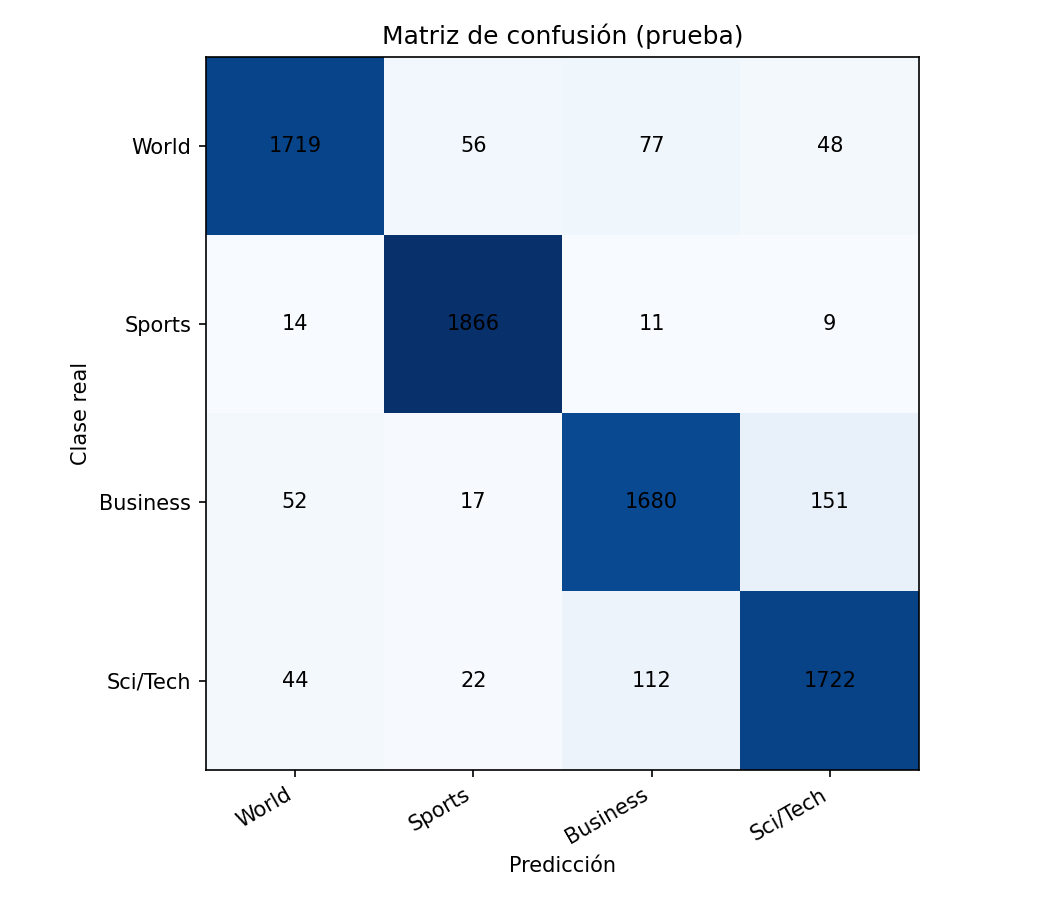
\includegraphics[width=\columnwidth]{../experiments/confusion_matrix.png}
\caption{Matriz de confusión en prueba, filas reales y columnas predichas.
Fuente: ejecución final del proyecto.}
\label{fig:matrix}
\end{figure}
\begin{figure}[t]
\centering
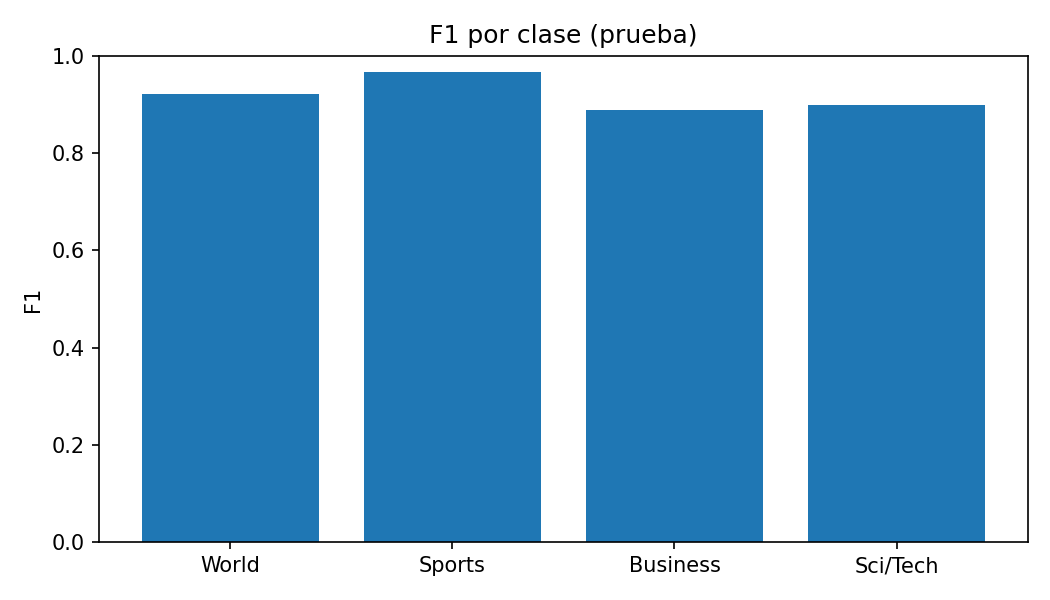
\includegraphics[width=\columnwidth]{../experiments/f1_per_class.png}
\caption{F1 por clase en prueba. Fuente: ejecución final del proyecto.}
\label{fig:f1}
\end{figure}

La línea base histórica registró F1 macro de 0,9177 en prueba;
la diferencia aproximada frente a la configuración elegida es
0,15 puntos porcentuales, inferior al objetivo de 1 punto.
Como la línea base ya había consultado prueba, esta cifra solo
sirve como referencia descriptiva y no reemplaza la comparación
entre configuraciones en validación. No se calcularon intervalos
bootstrap ni la prueba de McNemar; no se afirma significancia
estadística.

\subsection{Costo computacional y estimaciones ambientales}
Se midieron ejecuciones con \texttt{OfflineEmissionsTracker} de
CodeCarbon, en modo \texttt{process}, país COL e intervalo de un
segundo. Durante la validación, el ganador consumió alrededor de
0,0007175 kWh y emitió 0,0001340 kg CO\(_2\)eq, con 70,04 segundos
de ajuste y 1,64 de predicción. La regresión logística de unigramas
registró 0,0001842 kWh y 0,0000344 kg CO\(_2\)eq;
ComplementNB, 0,0001239 kWh y 0,0000231 kg CO\(_2\)eq; y
SGDClassifier, 0,0001356 kWh y 0,0000253 kg CO\(_2\)eq.
La alternativa más eficiente en este grupo no necesariamente
ofrece el F1 macro más alto.

En la ejecución final se midieron 118,31 segundos de ajuste y
1,32 de predicción. \texttt{run\_config.json} y el último registro
de \texttt{experiments/carbon/final\_model.csv} coinciden en
0,0011500 kWh y 0,0002148 kg CO\(_2\)eq (aproximadamente
0,2148 gramos). El CSV conserva también mediciones de otras
ejecuciones que no deben confundirse con esta. Las magnitudes
ambientales son estimaciones sujetas al hardware, carga del equipo,
sistema operativo, versión de Python y CodeCarbon, duración e
intensidad de carbono utilizada para Colombia; no deben
generalizarse como propiedades intrínsecas del algoritmo.

\subsection{Revisión de errores}
Se extrajeron 20 errores de distintos pares de clases; Anderson
revisó diez fragmentos y registró las categorías y limitaciones
en \texttt{experiments/error\_review\_confirmed.json} el 27 de
noviembre de 2026. Para la discusión se agrupan por límite
observado, sin reproducir noticias:
\begin{itemize}
\item Cuatro cruces temáticos (índices 36, 126, 264 y 1840):
 política y petróleo, seguridad olímpica, hallazgo histórico con
 referencias geográficas y deporte con lenguaje financiero. La
 categoría depende de reconocer el tema principal entre pistas
 concurrentes.
\item Tres predicciones sin relación deportiva o tecnológica clara
 con el tema visible (3, 41 y 1613): un pronóstico de incendios,
 una noticia comercial y un caso de Craigslist. Términos como
 ``park'' y ``run'' en el último describen actividades con un
 perro, sin que ello pruebe qué características pesaron en el modelo.
\item Tres casos con contexto insuficiente o etiqueta difícil
 de verificar (155, 344 y 408): temas de salud/cultura, un
 fragmento sin pistas deportivas suficientes y un texto político
 etiquetado Business que parece compatible con World. No se
 declara errónea la etiqueta de referencia sin ver el contexto
 ausente.
\end{itemize}
Cada una de las diez categorías de revisión corresponde a un caso.
El conjunto independiente de doce borradores propuestos por IA
no se cuenta como revisión humana adicional. Los posibles motivos
son hipótesis: no se analizaron los pesos del modelo para demostrar
la causa de una decisión individual.

\section{Limitaciones, uso responsable y reproducibilidad}
Las cuatro etiquetas son una taxonomía limitada y varios textos
contienen temas simultáneos. El corpus es de noticias antiguas
en inglés, con posibles sesgos editoriales, temporales y
geográficos; la exactitud en este banco de prueba no respalda
el uso sobre noticias actuales o en español sin una evaluación
específica. Tampoco justifica moderación automática, verificación
de hechos, decisiones financieras o priorización de personas.
La probabilidad que muestra el prototipo no explica causalmente
la clasificación ni valida la veracidad de una noticia.

Los parámetros y métricas de validación están en
\texttt{experiments/model\_comparison.csv}; la repetición en
\texttt{experiments/stability.csv}; y la prueba, matriz y estimación
final en \texttt{experiments/run\_config.json}. El modelo y los
errores con textos no se distribuyen. Para reproducir el
entrenamiento se recomienda Python 3.11 y las dependencias
fijadas en el repositorio. Los tiempos, y en especial las
estimaciones ambientales, no se esperan idénticos en otro equipo.

\section{Conclusiones}
Para las cuatro configuraciones examinadas, ComplementNB y
SGDClassifier no superaron la regresión logística en F1 macro
de validación. Los bigramas mejoraron aproximadamente 0,21
puntos porcentuales a costa de mayor tiempo de entrenamiento.
El modelo elegido obtuvo 0,9192 de F1 macro en prueba, sin
alcanzar la mejora de un punto porcentual frente a la línea base
histórica. Los diez casos revisados ilustran cruces de temas,
contexto insuficiente y discrepancias que no pueden explicarse
mediante la probabilidad de predicción por sí sola.

\section*{Contribuciones y uso de IA}
La contribución individual de los autores está pendiente de
confirmación. Se utilizó IA como apoyo en estructura, código,
documentación y propuestas de hipótesis para algunos casos.
Anderson revisó y registró diez casos; las sugerencias de IA
no sustituyen esa revisión ni prueban las causas del error.

\begin{thebibliography}{7}
\bibitem{zhang} X. Zhang, J. Zhao y Y. LeCun, ``Character-level
Convolutional Networks for Text Classification,'' en
\emph{Advances in Neural Information Processing Systems 28
(NIPS 2015)}, 2015. [En línea]. Disponible:
\url{https://arxiv.org/abs/1509.01626}
\bibitem{rennie} J. D. M. Rennie, L. Shih, J. Teevan y D. R. Karger,
``Tackling the Poor Assumptions of Naive Bayes Text Classifiers,''
en \emph{Proc. 20th Int. Conf. Machine Learning (ICML)},
pp. 616--623, 2003. [En línea]. Disponible:
\url{https://people.csail.mit.edu/jrennie/papers/icml03-nb.pdf}
\bibitem{joachims} T. Joachims, ``Text Categorization with Support
Vector Machines: Learning with Many Relevant Features,'' en
\emph{Machine Learning: ECML-98}, LNCS 1398, pp. 137--142,
Springer, 1998, doi: 10.1007/BFb0026683.
\bibitem{pedregosa} F. Pedregosa \emph{et al.},
``Scikit-learn: Machine Learning in Python,'' \emph{J. Mach.
Learn. Res.}, vol. 12, no. 85, pp. 2825--2830, 2011.
[En línea]. Disponible: \url{https://jmlr.org/papers/v12/pedregosa11a.html}
\bibitem{russell} S. Russell y P. Norvig,
\emph{Artificial Intelligence: A Modern Approach}, 4.a ed.
Pearson, 2020, ISBN 978-0-13-461099-3.
\bibitem{agnews} Hugging Face, ``AG News (fancyzhx/ag\_news),''
conjunto de datos en línea. [En línea]. Disponible:
\url{https://huggingface.co/datasets/fancyzhx/ag_news}
[Consultado: 27-nov-2026].
\bibitem{gulli} A. Gulli, ``AG's corpus of news articles,''
Universidad de Pisa. [En línea]. Disponible:
\url{https://www.di.unipi.it/~gulli/AG_corpus_of_news_articles.html}
[Consultado: 27-nov-2026].
\end{thebibliography}
\end{document}
